
\chapter{公式、图表和插图}
\label{chap:eqnFigAndTab}

\section{公式及术语表}
\label{sec:eqn}

\begin{equation}
 \label{eqn:LBmodel}
   C_{L}=C_{L0}+C_{L\alpha }\left ( \frac{1+\sqrt{X}}{2} \right )\alpha 
\end{equation}
\nomenclature{$t$}{Time}%
\nomenclature{$\alpha$}{Angle of attack (AoA)}%
\nomenclature{$\dot{\alpha}$}{Time rate of change of AoA}%
\nomenclature{$C_{L\alpha}$}{Lift curve slope}%
\nomenclature{$C_{L0}$}{Lift coefficient at $\alpha=0^{\circ}$}%
\nomenclature{$X$}{Chordwise location of unsteady flow separation point}%
\nomenclature{$a_{1}$}{Coefficient of the flow separation function}%
\nomenclature{$\alpha^{\star}$}{AoA at which $X=0.5$ }%
\nomenclature{$\tau _{1},\tau _{2}$}{Time constants of the flow separation function}%

\section{表格}
\label{sec:tab}

\begin{table}                % no placement specified: defaults to here, top, bottom, page
\centering
 \begin{center}
  \caption{Physical meaning of parameters in L-B model.\cite{Pattinson:2013_postall_oscillation}}
  \label{tab:LB-parameters}
  \begin{tabular}{cl}
       \\\hline
       Parameters & Physical meaning       \\\hline
       $C_{L\alpha}$ & Lift curve slope \\
       $a_{1}$ & Controls the shape of the stall curve \\
       $\alpha^{\star}$ & The break point at which $X=0.5$ \\
       $\tau_{1}$ & Represents the tendency of the model to track the static curve \\
       $\tau_{2}$ & Gives the model lift overshoot \\\hline
  \end{tabular}
 \end{center}
\end{table}

\section{插图}
\label{sec:fig}


\begin{figure}
\centering
   \includegraphics[width=12cm]{./img/visual_jpg}
   %\includegraphics[width=6cm,height=5cm]{./img/visual_jpg}
  \caption{插入一个jpg图片}
  \label{fig:visual}
\end{figure}

\begin{figure}
\centering
   \includegraphics[width=10cm]{./img/Geom_pdf}
  \caption{插入一个pdf图片}
  \label{fig:visual}
\end{figure}

\begin{figure}
\centering
 \begin{subfigmatrix}{2}                 % number of columns
  \subfigure[jpg格式图片]{\includegraphics[width=6cm]{./img/Curve_jpg}
  \label{fig:subfig:Curve_jpg}}
  \subfigure[eps格式图片]{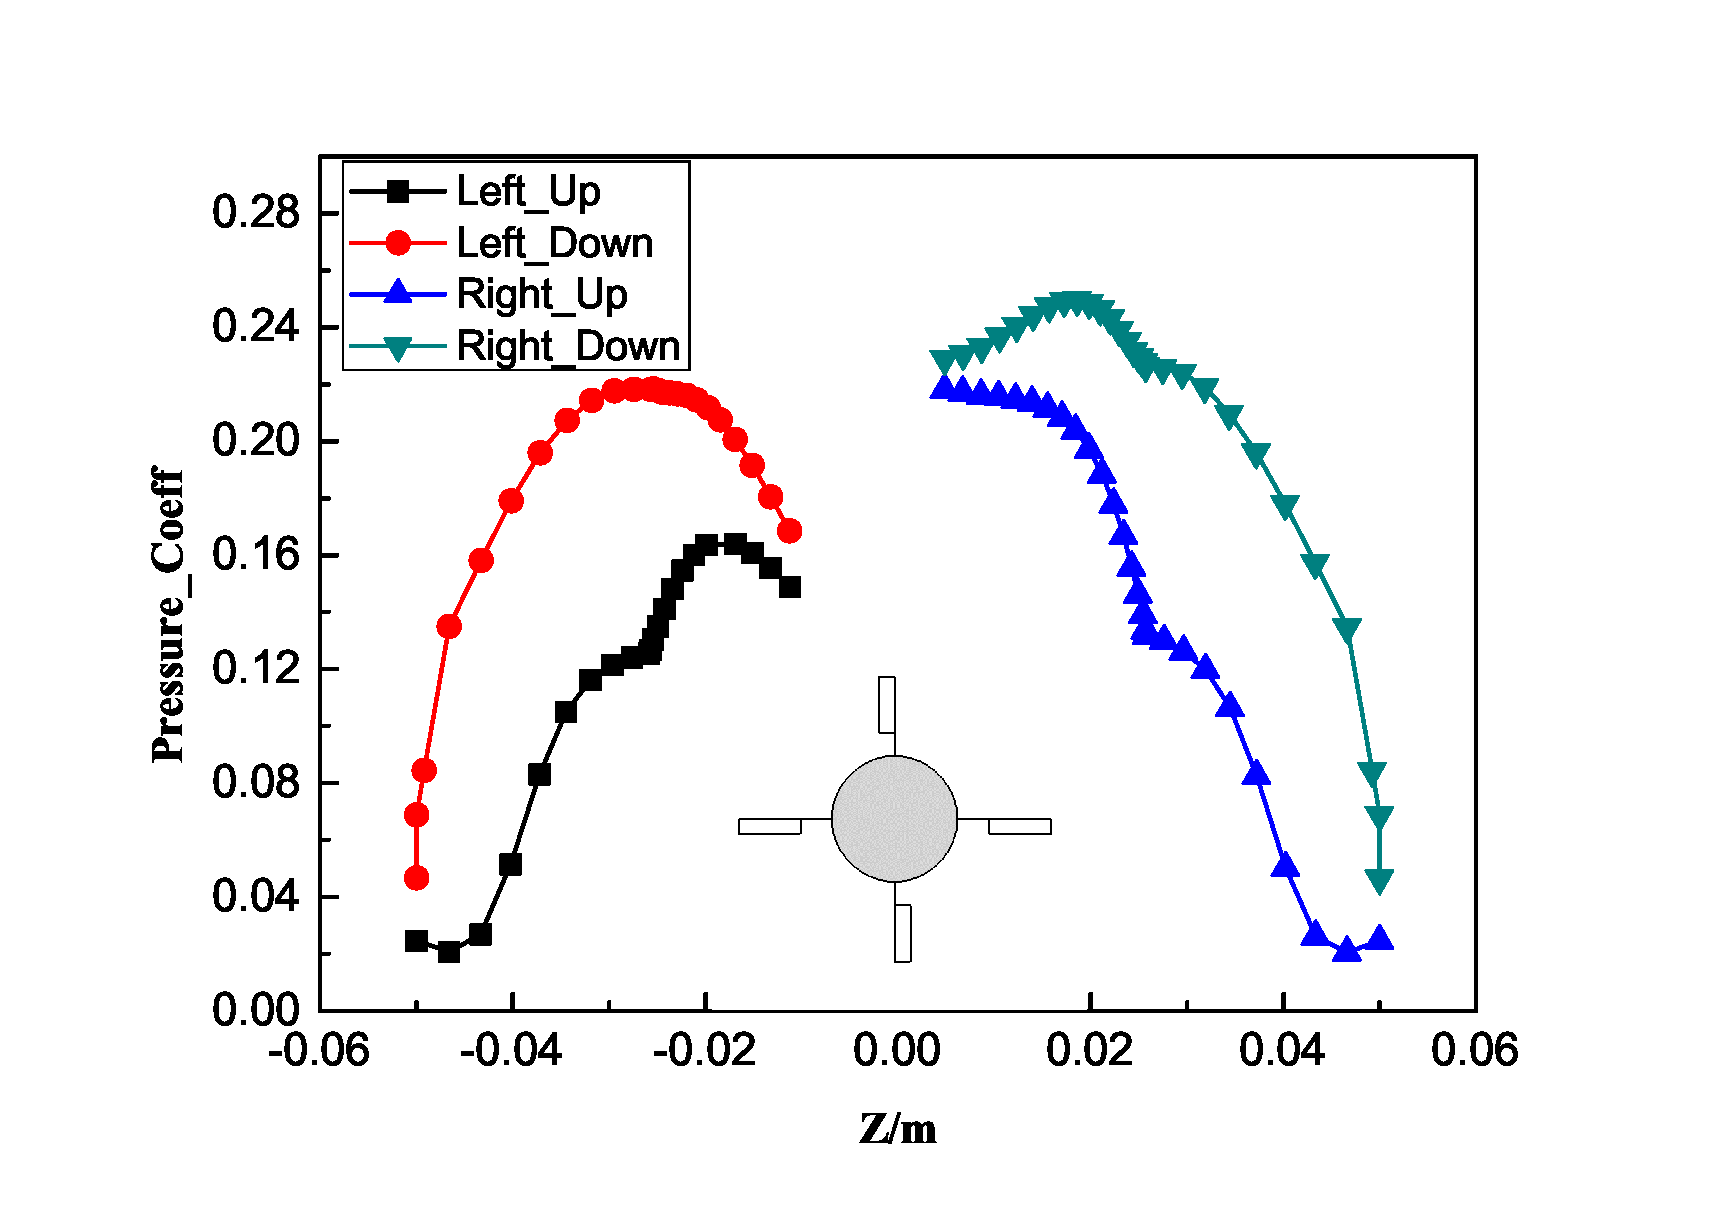
\includegraphics[width=6.5cm]{./img/plot_eps.eps}
  \label{fig:subfig:plot_eps}}
 \end{subfigmatrix}
 \caption{插入横排两列图片:a) jpg位图格式;b) eps矢量图格式}
 \label{fig:dynamic}
\end{figure}
